\begin{figure}[H]
	\centering
	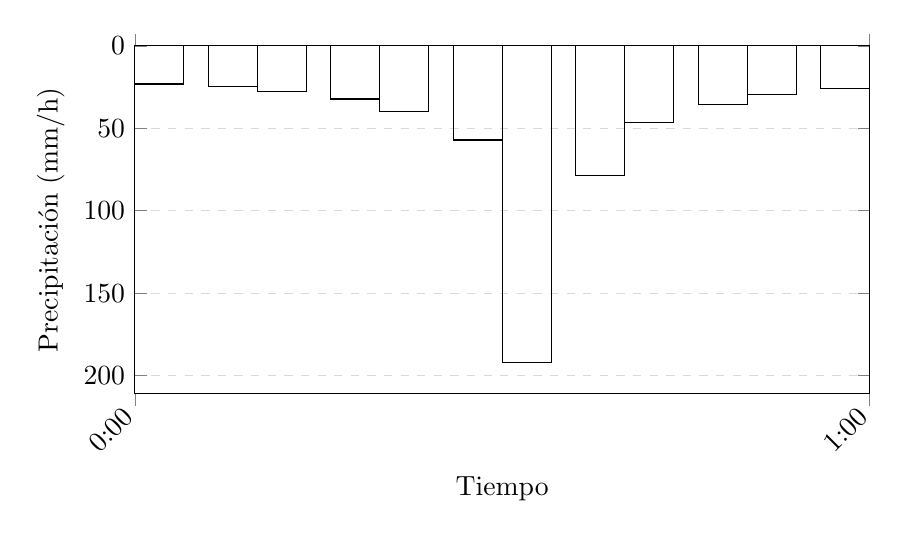
\begin{tikzpicture}
		\begin{axis}[
			width=0.9\textwidth,
			height=6cm,
			xlabel={Tiempo},
			ylabel={Precipitación (mm/h)},
			y dir=reverse,
			ymin=0,
			ymax=211,
			xmin=0,
			xmax=60,
			ybar,
			bar width=4,
			xtick={0, 60},
			xticklabels={0:00, 1:00},
			xticklabel style={rotate=45, anchor=east},
			grid=major,
			grid style={dashed, gray!30},
			]
			\addplot [
			draw=black,
			fill=none
			]
			coordinates {
				(2, 23.16) (8, 24.60) (12, 27.72) (18, 32.28) (22, 40.08)
				(28, 57.12) (32, 192.00) (38, 78.72) (42, 46.56) (48, 35.64)
				(52, 29.76) (58, 25.92)
			};
		\end{axis}
	\end{tikzpicture}
	\caption{Hietograma - BLOCKS $T_r$=10 años (P=51.1 mm)}
	\label{fig:hyeto_kirpich_blocks_Tr10}
\end{figure}
